\documentclass[leqno, 12pt]{article}
\usepackage{tikz}
\usepackage{amsmath}
\usepackage{ulem}
\usetikzlibrary{angles,quotes,intersections,arrows.meta,calc}
\usepackage[a4paper, portrait, margin=1cm]{geometry}
\usepackage{multicol}
\usepackage{fancyhdr}

\def \HeadingAnswers {\section*{\Large Name: \underline{\hspace{8cm}} \hfill Date: \underline{\hspace{3cm}}} \vspace{-3mm}
{Parallel lines : Answers} \vspace{1pt}\hrule}

% raise footer with page number; no header
\fancypagestyle{myfancypagestyle}{
  \fancyhf{}% clear all header and footer fields
  \renewcommand{\headrulewidth}{0pt} % no rule under header
  \fancyfoot[C] {\thepage} \setlength{\footskip}{14.5pt} % raise page number 6pt
}
\pagestyle{myfancypagestyle}  % apply myfancypagestyle

\newcounter{minipagecount}

\begin{document}
\HeadingAnswers
\begin{multicols}{2}


\begin{equation}
  \text{a} = \text{61}^\circ
  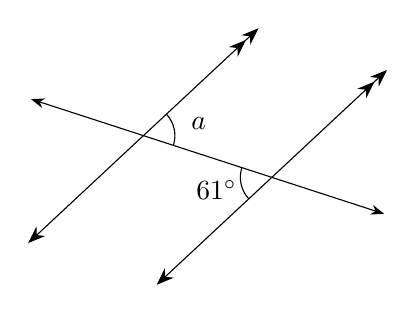
\begin{tikzpicture}[scale=1.0, baseline=(current bounding box.north)]
    \begin{scope}[rotate=342]
      % Draw the first line
      \draw[<->>, >={Stealth[scale=1.3]}, name path=P1] (0, 0) -- (1.9392384809853485, 3.498478828557583);
      % Draw the second line with the calculated offsets
      \draw[<->>, >={Stealth[scale=1.3]}, name path=P2] (1.7150311018099802, 0) -- (3.6542695827953287, 3.498478828557583);
      % Draw the transversal through the middle of the parallel lines
      \draw[<->, >=Stealth, name path=P3] (-0.530380759507326, 1.7492394142787915) -- (4.184650342302655, 1.7492394142787915);
      \path [name intersections={of=P1 and P3,by=A}];
      \path [name intersections={of=P2 and P3,by=B}];
      % Draw the angle
      \coordinate (p1s) at (0, 0);
      \coordinate (p1e) at (1.9392384809853485, 3.498478828557583);
      \coordinate (p2s) at (1.7150311018099802, 0);
      \coordinate (p2e) at (3.6542695827953287, 3.498478828557583);
      \coordinate (ts) at (-0.530380759507326, 1.7492394142787915);
      \coordinate (te) at (4.184650342302655, 1.7492394142787915);
      \draw pic["$a$", draw=black, -, angle eccentricity=1.8, angle radius=0.4cm] {angle=te--A--p1e};
\draw pic["$61^\circ$", draw=black, -, angle eccentricity=1.8, angle radius=0.4cm] {angle=ts--B--p2s};

    \end{scope}
  \end{tikzpicture}
\end{equation}\vspace{1cm}
\begin{equation}
  \text{a} = \text{48}^\circ
  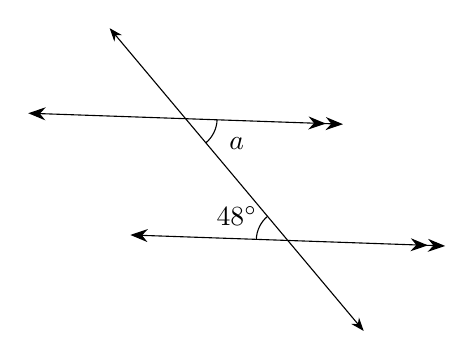
\begin{tikzpicture}[scale=1.0, baseline=(current bounding box.north)]
    \begin{scope}[rotate=310]
      % Draw the first line
      \draw[<->>, >={Stealth[scale=1.3]}, name path=P1] (0, 0) -- (2.676522425435433, 2.972579301909577);
      % Draw the second line with the calculated offsets
      \draw[<->>, >={Stealth[scale=1.3]}, name path=P2] (2.018449094409564, 0) -- (4.694971519844997, 2.972579301909577);
      % Draw the transversal through the middle of the parallel lines
      \draw[<->, >=Stealth, name path=P3] (-0.16173878728228352, 1.4862896509547885) -- (4.856710307127281, 1.4862896509547885);
      \path [name intersections={of=P1 and P3,by=A}];
      \path [name intersections={of=P2 and P3,by=B}];
      % Draw the angle
      \coordinate (p1s) at (0, 0);
      \coordinate (p1e) at (2.676522425435433, 2.972579301909577);
      \coordinate (p2s) at (2.018449094409564, 0);
      \coordinate (p2e) at (4.694971519844997, 2.972579301909577);
      \coordinate (ts) at (-0.16173878728228352, 1.4862896509547885);
      \coordinate (te) at (4.856710307127281, 1.4862896509547885);
      \draw pic["$a$", draw=black, -, angle eccentricity=1.8, angle radius=0.4cm] {angle=te--A--p1e};
\draw pic["$48^\circ$", draw=black, -, angle eccentricity=1.8, angle radius=0.4cm] {angle=ts--B--p2s};

    \end{scope}
  \end{tikzpicture}
\end{equation}\vspace{1cm}
\begin{equation}
  \text{a} = \text{61}^\circ
  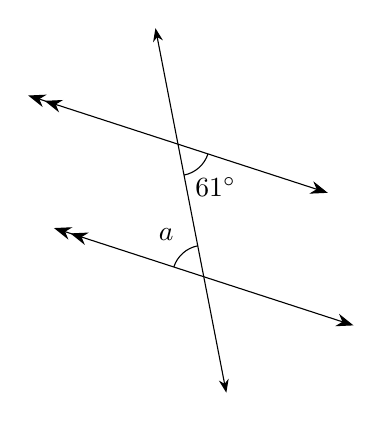
\begin{tikzpicture}[scale=1.0, baseline=(current bounding box.north)]
    \begin{scope}[rotate=101]
      % Draw the first line
      \draw[<->>, >={Stealth[scale=1.3]}, name path=P1] (0, 0) -- (1.9392384809853485, 3.498478828557583);
      % Draw the second line with the calculated offsets
      \draw[<->>, >={Stealth[scale=1.3]}, name path=P2] (1.7150311018099802, 0) -- (3.6542695827953287, 3.498478828557583);
      % Draw the transversal through the middle of the parallel lines
      \draw[<->, >=Stealth, name path=P3] (-0.530380759507326, 1.7492394142787915) -- (4.184650342302655, 1.7492394142787915);
      \path [name intersections={of=P1 and P3,by=A}];
      \path [name intersections={of=P2 and P3,by=B}];
      % Draw the angle
      \coordinate (p1s) at (0, 0);
      \coordinate (p1e) at (1.9392384809853485, 3.498478828557583);
      \coordinate (p2s) at (1.7150311018099802, 0);
      \coordinate (p2e) at (3.6542695827953287, 3.498478828557583);
      \coordinate (ts) at (-0.530380759507326, 1.7492394142787915);
      \coordinate (te) at (4.184650342302655, 1.7492394142787915);
      \draw pic["$a$", draw=black, -, angle eccentricity=1.8, angle radius=0.4cm] {angle=te--A--p1e};
\draw pic["$61^\circ$", draw=black, -, angle eccentricity=1.8, angle radius=0.4cm] {angle=ts--B--p2s};

    \end{scope}
  \end{tikzpicture}
\end{equation}\vspace{1cm}
\begin{equation}
  \text{g} = \text{53}^\circ
  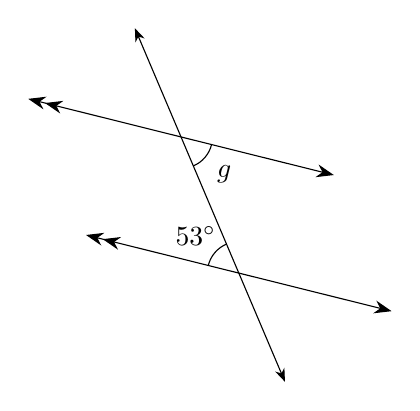
\begin{tikzpicture}[scale=1.0, baseline=(current bounding box.north)]
    \begin{scope}[rotate=113]
      % Draw the first line
      \draw[<->>, >={Stealth[scale=1.3]}, name path=P1] (0, 0) -- (2.4072600926081935, 3.1945420401891713);
      % Draw the second line with the calculated offsets
      \draw[<->>, >={Stealth[scale=1.3]}, name path=P2] (1.8782034872343385, 0) -- (4.285463579842532, 3.1945420401891713);
      % Draw the transversal through the middle of the parallel lines
      \draw[<->, >=Stealth, name path=P3] (-0.296369953695903, 1.5972710200945857) -- (4.581833533538435, 1.5972710200945857);
      \path [name intersections={of=P1 and P3,by=A}];
      \path [name intersections={of=P2 and P3,by=B}];
      % Draw the angle
      \coordinate (p1s) at (0, 0);
      \coordinate (p1e) at (2.4072600926081935, 3.1945420401891713);
      \coordinate (p2s) at (1.8782034872343385, 0);
      \coordinate (p2e) at (4.285463579842532, 3.1945420401891713);
      \coordinate (ts) at (-0.296369953695903, 1.5972710200945857);
      \coordinate (te) at (4.581833533538435, 1.5972710200945857);
      \draw pic["$g$", draw=black, -, angle eccentricity=1.8, angle radius=0.4cm] {angle=ts--B--p2s};
\draw pic["$53^\circ$", draw=black, -, angle eccentricity=1.8, angle radius=0.4cm] {angle=te--A--p1e};

    \end{scope}
  \end{tikzpicture}
\end{equation}\vspace{1cm}
\begin{equation}
  \text{d} = \text{99}^\circ
  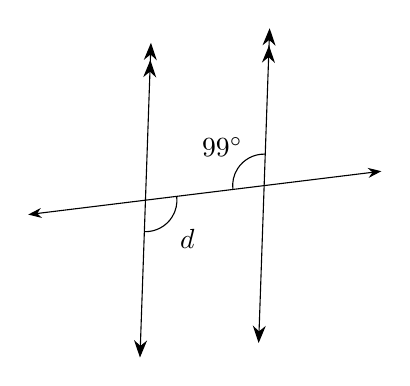
\begin{tikzpicture}[scale=1.0, baseline=(current bounding box.north)]
    \begin{scope}[rotate=7]
      % Draw the first line
      \draw[<->>, >={Stealth[scale=1.3]}, name path=P1] (0, 0) -- (0.6257378601609237, 3.950753362380551);
      % Draw the second line with the calculated offsets
      \draw[<->>, >={Stealth[scale=1.3]}, name path=P2] (1.5186976886820043, 0) -- (2.144435548842928, 3.950753362380551);
      % Draw the transversal through the middle of the parallel lines
      \draw[<->, >=Stealth, name path=P3] (-1.187131069919538, 1.9753766811902755) -- (3.331566618762466, 1.9753766811902755);
      \path [name intersections={of=P1 and P3,by=A}];
      \path [name intersections={of=P2 and P3,by=B}];
      % Draw the angle
      \coordinate (p1s) at (0, 0);
      \coordinate (p1e) at (0.6257378601609237, 3.950753362380551);
      \coordinate (p2s) at (1.5186976886820043, 0);
      \coordinate (p2e) at (2.144435548842928, 3.950753362380551);
      \coordinate (ts) at (-1.187131069919538, 1.9753766811902755);
      \coordinate (te) at (3.331566618762466, 1.9753766811902755);
      \draw pic["$d$", draw=black, -, angle eccentricity=1.8, angle radius=0.4cm] {angle=p1s--A--te};
\draw pic["$99^\circ$", draw=black, -, angle eccentricity=1.8, angle radius=0.4cm] {angle=p2e--B--ts};

    \end{scope}
  \end{tikzpicture}
\end{equation}\vspace{1cm}
\begin{equation}
  \text{a} = \text{128}^\circ
  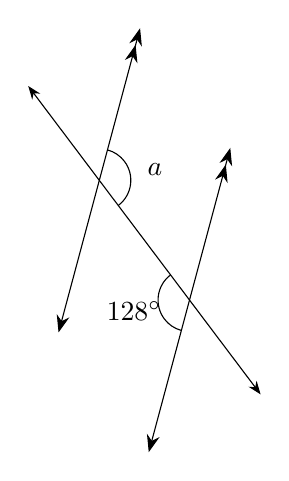
\begin{tikzpicture}[scale=1.0, baseline=(current bounding box.north)]
    \begin{scope}[rotate=307]
      % Draw the first line
      \draw[<->>, >={Stealth[scale=1.3]}, name path=P1] (0, 0) -- (-2.462645901302633, 3.152043014426888);
      % Draw the second line with the calculated offsets
      \draw[<->>, >={Stealth[scale=1.3]}, name path=P2] (1.903527322608868, 0) -- (-0.5591185786937651, 3.152043014426888);
      % Draw the transversal through the middle of the parallel lines
      \draw[<->, >=Stealth, name path=P3] (-2.7313229506513164, 1.576021507213444) -- (2.1722043719575517, 1.576021507213444);
      \path [name intersections={of=P1 and P3,by=A}];
      \path [name intersections={of=P2 and P3,by=B}];
      % Draw the angle
      \coordinate (p1s) at (0, 0);
      \coordinate (p1e) at (-2.462645901302633, 3.152043014426888);
      \coordinate (p2s) at (1.903527322608868, 0);
      \coordinate (p2e) at (-0.5591185786937651, 3.152043014426888);
      \coordinate (ts) at (-2.7313229506513164, 1.576021507213444);
      \coordinate (te) at (2.1722043719575517, 1.576021507213444);
      \draw pic["$a$", draw=black, -, angle eccentricity=1.8, angle radius=0.4cm] {angle=te--A--p1e};
\draw pic["$128^\circ$", draw=black, -, angle eccentricity=1.8, angle radius=0.4cm] {angle=ts--B--p2s};

    \end{scope}
  \end{tikzpicture}
\end{equation}\vspace{1cm}
\begin{equation}
  \text{f} = \text{63}^\circ
  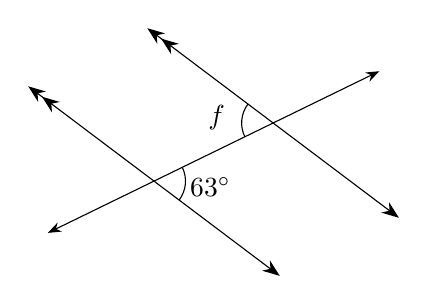
\begin{tikzpicture}[scale=1.0, baseline=(current bounding box.north)]
    \begin{scope}[rotate=26]
      % Draw the first line
      \draw[<->>, >={Stealth[scale=1.3]}, name path=P1] (0, 0) -- (-1.815961998958187, 3.5640260967534716);
      % Draw the second line with the calculated offsets
      \draw[<->>, >={Stealth[scale=1.3]}, name path=P2] (1.6834893564515412, 0) -- (-0.1324726425066458, 3.5640260967534716);
      % Draw the transversal through the middle of the parallel lines
      \draw[<->, >=Stealth, name path=P3] (-2.4079809994790935, 1.7820130483767358) -- (2.2755083569724475, 1.7820130483767358);
      \path [name intersections={of=P1 and P3,by=A}];
      \path [name intersections={of=P2 and P3,by=B}];
      % Draw the angle
      \coordinate (p1s) at (0, 0);
      \coordinate (p1e) at (-1.815961998958187, 3.5640260967534716);
      \coordinate (p2s) at (1.6834893564515412, 0);
      \coordinate (p2e) at (-0.1324726425066458, 3.5640260967534716);
      \coordinate (ts) at (-2.4079809994790935, 1.7820130483767358);
      \coordinate (te) at (2.2755083569724475, 1.7820130483767358);
      \draw pic["$f$", draw=black, -, angle eccentricity=1.8, angle radius=0.4cm] {angle=p2e--B--ts};
\draw pic["$63^\circ$", draw=black, -, angle eccentricity=1.8, angle radius=0.4cm] {angle=p1s--A--te};

    \end{scope}
  \end{tikzpicture}
\end{equation}\vspace{1cm}
\begin{equation}
  \text{f} = \text{117}^\circ
  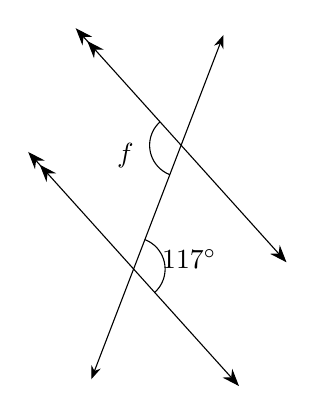
\begin{tikzpicture}[scale=1.0, baseline=(current bounding box.north)]
    \begin{scope}[rotate=69]
      % Draw the first line
      \draw[<->>, >={Stealth[scale=1.3]}, name path=P1] (0, 0) -- (1.8159619989581872, 3.564026096753471);
      % Draw the second line with the calculated offsets
      \draw[<->>, >={Stealth[scale=1.3]}, name path=P2] (1.6834893564515414, 0) -- (3.499451355409729, 3.564026096753471);
      % Draw the transversal through the middle of the parallel lines
      \draw[<->, >=Stealth, name path=P3] (-0.5920190005209061, 1.7820130483767356) -- (4.091470355930635, 1.7820130483767356);
      \path [name intersections={of=P1 and P3,by=A}];
      \path [name intersections={of=P2 and P3,by=B}];
      % Draw the angle
      \coordinate (p1s) at (0, 0);
      \coordinate (p1e) at (1.8159619989581872, 3.564026096753471);
      \coordinate (p2s) at (1.6834893564515414, 0);
      \coordinate (p2e) at (3.499451355409729, 3.564026096753471);
      \coordinate (ts) at (-0.5920190005209061, 1.7820130483767356);
      \coordinate (te) at (4.091470355930635, 1.7820130483767356);
      \draw pic["$f$", draw=black, -, angle eccentricity=1.8, angle radius=0.4cm] {angle=p2e--B--ts};
\draw pic["$117^\circ$", draw=black, -, angle eccentricity=1.8, angle radius=0.4cm] {angle=p1s--A--te};

    \end{scope}
  \end{tikzpicture}
\end{equation}\vspace{1cm}

\end{multicols}
\end{document}

